%!TeX spellcheck = sl_SI
% vim: set spell spelllang=sl:
% za preverjanje črkovanja, če se uporablja Texstudio ali vim
\documentclass[12pt,a4paper,twoside]{article}
\usepackage[utf8]{inputenc}  % pravilno razpoznavanje unicode znakov

% NASLEDNJE UKAZE USTREZNO POPRAVI
\newcommand{\program}{Matematika} % ime studijskega programa
\newcommand{\imeavtorja}{Miha Avsec} % ime avtorja
\newcommand{\imementorja}{doc.~dr.~Anita Buckley} % akademski naziv in ime mentorja, uporabi poln naziv, prof.~dr.~, doc.~dr., ali izr.~prof.~dr.
\newcommand{\imesomentorja}{pred.~mag.~Matjaž Praprotnik} % akademski naziv in ime somentorja, če ga imate
\newcommand{\naslovdela}{Kubične krivulje v kriptografiji}
\newcommand{\letnica}{2019} % letnica magistriranja
\newcommand{\opis}{??.}  % Opis dela v eni povedi. Ne sme vsebovati matematičnih simbolov v $ $.
\newcommand{\kljucnebesede}{kubična krivulja \sep kriptografija \sep ...} % ključne besede, ločene z \sep, da se PDF metapodatki prav procesirajo
\newcommand{\keywords}{cubic curve \sep cryptography} % ključne besede v angleščini
\newcommand{\organization}{Univerza v Ljubljani, Fakulteta za matematiko in fiziko} % fakulteta
\newcommand{\literatura}{literatura}  % pot do datoteke z literaturo (brez .bib končnice)
\newcommand{\sep}{, }  % separator med ključnimi besedami v besedilu
% KONEC PODATKOV

\usepackage{bibentry}         % za navajanje literature v programu dela s celim imenom
\nobibliography{\literatura}
\newcommand{\plancite}[1]{\item[\cite{#1}] \bibentry{#1}} % citiranje v programu dela

\usepackage{filecontents}  % za pisanje datoteke s PDF metapodatki
\usepackage{silence} \WarningFilter{latex}{Overwriting file}  % odstrani annoying warning o obstoju datoteke
% datoteka s PDF metapodatki, zgenerira se kot magisterij.xmpdata
\begin{filecontents*}{\jobname.xmpdata}
  \Title{\naslovdela}
  \Author{\imeavtorja}
  \Keywords{\kljucnebesede}
  \Subject{\opis}
  \Org{\organization}
\end{filecontents*}

\usepackage[a-1b]{pdfx}  % zgenerira PDF v tem PDF/A-1b formatu, kot zahteva knjižnica
\hypersetup{bookmarksopen, bookmarksdepth=3, colorlinks=true,
  linkcolor=black, anchorcolor=black, citecolor=black, filecolor=black,
  menucolor=black, runcolor=black, urlcolor=black, pdfencoding=auto,
  breaklinks=true, psdextra}

\usepackage[slovene]{babel}  % slovenščina
\usepackage[T1]{fontenc}     % naprednejše kodiranje fonta
\usepackage{amsmath,amssymb,amsfonts,amsthm} % matematični paketi
\usepackage[]{color} % barve
\usepackage{graphicx}     % za slike
\usepackage{emptypage}    % prazne strani so neoštevilčene, ampak so štete
\usepackage{units}        % fizikalne enote kot \unit[12]{kg} z polovico nedeljivega presledka, glej primer v kodi
\usepackage{makeidx}      % za stvarno kazalo, lahko zakomentiraš, če ne rabiš
\makeindex                % za stvarno kazalo, lahko zakomentiraš, če ne rabiš
% oblika strani
\usepackage[
  top=3cm,
  bottom=3cm,
  inner=3.5cm,      % margini za dvostransko tiskanje
  outer=2.5cm,
  footskip=40pt     % pozicija številke strani
]{geometry}

% VEČ ZANIMIVIH PAKETOV
% \usepackage{array}      % več možnosti za tabele
% \usepackage[list=true,listformat=simple]{subcaption}  % več kot ena slika na figure, omogoči slika 1a, slika 1b
% \usepackage[all]{xy}    % diagrami
% \usepackage{doi}        % za clickable DOI entrye v bibliografiji
% \usepackage{enumerate}     % več možnosti za sezname

% Za barvanje source kode
% \usepackage{minted}
% \renewcommand\listingscaption{Program}

% Za pisanje psevdokode
% \usepackage{algpseudocode}  % za psevdokodo
\usepackage{algorithm}
\floatname{algorithm}{Algoritem}
\renewcommand{\listalgorithmname}{Kazalo algoritmov}

% DRUGI TVOJI PAKETI:
% tukaj
 \usepackage{algorithmicx}



\setlength{\overfullrule}{50pt} % označi predlogo vrstico
\pagestyle{plain}               % samo številka strani na dnu, nobene glave / noge

% ukazi za matematična okolja
\theoremstyle{definition} % tekst napisan pokončno
\newtheorem{definicija}{Definicija}[section]
\newtheorem{primer}[definicija]{Primer}
\newtheorem{opomba}[definicija]{Opomba}
\newtheorem{aksiom}{Aksiom}

\theoremstyle{plain} % tekst napisan poševno
\newtheorem{lema}[definicija]{Lema}
\newtheorem{izrek}[definicija]{Izrek}
\newtheorem{trditev}[definicija]{Trditev}
\newtheorem{posledica}[definicija]{Posledica}

\numberwithin{equation}{section}  % števec za enačbe zgleda kot (2.7) in se resetira v vsakem poglavju

% Matematični ukazi
\newcommand{\R}{\mathbb R}
\newcommand{\N}{\mathbb N}
\newcommand{\Z}{\mathbb Z}
\renewcommand{\C}{\mathbb C}
\newcommand{\Q}{\mathbb Q}

\newcommand{\F}{\mathbb F}
\newcommand{\Fq}[1]{{\mathbb{F}_{#1}}}
\newcommand{\PP}{\mathbb P}
\newcommand{\E}[1]{E({#1})}
\newcommand{\MOD}[1]{\ \text{(mod }{#1}\text{)}}
% \DeclareMathOperator{\tr}{tr}  % morda potrebuješ operator za sled ali kaj drugega?

% bold matematika znotraj \textbf{ }, tudi v naslovih, kot \omega spodaj
\makeatletter \g@addto@macro\bfseries{\boldmath} \makeatother

% Poimenuj kazalo slik kot ``Kazalo slik'' in ne ``Slike''
\addto\captionsslovene{
  \renewcommand{\listfigurename}{Kazalo slik}%
}

% če želiš, da se poglavja začnejo na lihih straneh zgoraj
% \let\oldsection\section
% \def\section{\cleardoublepage\oldsection}

%%%%%%%%%%%%%%%%%%%%%%%%%%%%%%%%%%%%%%%%%%
%%%%%%           DOCUMENT           %%%%%%
%%%%%%%%%%%%%%%%%%%%%%%%%%%%%%%%%%%%%%%%%%

\begin{document}

\pagenumbering{roman} % začnemo z rimskimi številkami
\thispagestyle{empty} % ampak na prvi strani ni številke

\noindent{\large
UNIVERZA V LJUBLJANI\\[1mm]
FAKULTETA ZA MATEMATIKO IN FIZIKO\\[5mm]
\program\ -- 2.~stopnja}
% ustrezno dopolni za IŠRM
\vfill

\begin{center}
  \large
  \imeavtorja\\[3mm]
  \Large
  \textbf{\MakeUppercase{\naslovdela}}\\[10mm]
  \large
  Magistrsko delo \\[1cm]
  Mentor: \imementorja \\[2mm] % ustrezno popravi spol
   Somentor: \imesomentorja   % dodaj, če potrebno
\end{center}
\vfill

\noindent{\large Ljubljana, \letnica}

\cleardoublepage

%% IZJAVA O AVTORSTVU
%\pdfbookmark[1]{Izjava o avtorstvu}{izjava} % bookmark v PDF, \pdfbookmark[nivo]{text}{label}
%
%% izjava: po potrebi spremeni v žensko obliko
%\setlength\topsep{0pt}
%\setlength\parskip{0pt}
%\begin{center}
%  \textbf{Univerza v Ljubljani} \\
%  \textbf{Fakulteta za matematiko in fiziko}
%
%  \vfill
%
%  \underline{Izjava o avtorstvu, istovetnosti tiskane in elektronske verzije magistrskega dela in} \\
%  \underline{objavi osebnih podatkov študenta}
%
%  \vfill
%
%  \setlength\topsep{0pt}
%  \setlength\parskip{0pt}
%  \begin{flushleft}
%    Spodaj podpisani študent \imeavtorja{} avtor magistrskega dela (v nadaljevanju: pisnega
%    zaključnega dela študija) z naslovom:
%  \end{flushleft}
%
%  \vfill
%
%  \textbf{\naslovdela}
%
%  \vfill
%
%  IZJAVLJAM
%\end{center}
%
%\begin{enumerate}[1. ]
%  \item \emph{Obkrožite eno od variant a) ali b)}
%  \begin{enumerate}[a)]
%    \item da sem pisno zaključno delo študija izdelal samostojno;
%    \item da je pisno zaključno delo študija rezultat lastnega dela več kandidatov in izpolnjuje
%      pogoje, ki jih Statut UL določa za skupna zaključna dela študija ter je v zahtevanem deležu
%      rezultat mojega samostojnega dela;
%  \end{enumerate}
%  pod mentorstvom IZPOLNI. % dopiši \imementorja v rodilniku
%%   \\ in somentorstvom IZPOLNI. % dopiši \imesomentorja v rodilniku
%  \item da je tiskana oblika pisnega zaključnega dela študija istovetna elektronski obliki
%    pisnega zaključnega dela študija;
%  \item da sem pridobil vsa potrebna dovoljenja za uporabo podatkov in avtorskih del v pisnem
%    zaključnem delu študija in jih v pisnem zaključnem delu študija jasno označil;
%  \item da sem pri pripravi pisnega zaključnega dela študija ravnal v skladu z etičnimi načeli in,
%    kjer je to potrebno, za raziskavo pridobil soglasje etične komisije;
%  \item da soglašam, da se elektronska oblika pisnega zaključnega dela študija uporabi za preverjanje
%    podobnosti vsebine z drugimi deli s programsko  opremo za preverjanje podobnosti
%    vsebine, ki je povezana s študijskim informacijskim sistemom fakultete;
%  \item da na UL neodplačno, neizključno, prostorsko in časovno neomejeno prenašam pravico shranitve
%    avtorskega dela v elektronski obliki, pravico reproduciranja ter pravico dajanja pisnega
%    zaključnega dela študija na voljo javnosti na svetovnem spletu preko Repozitorija UL;
%  \item da dovoljujem objavo svojih osebnih podatkov, ki so navedeni v pisnem zaključnem delu študija
%    in tej izjavi, skupaj z objavo pisnega zaključnega dela študija.
%\end{enumerate}
%
%\vfill
%
%\noindent
%Kraj:  \hfill   Podpis študenta: \phantom{prostor za podpis}
%
%\vfill
%
%\noindent
%Datum:
%
%\cleardoublepage
%% END IZJAVA O AVTORSTVU

% zahvala
\pdfbookmark[1]{Zahvala}{zahvala} %
\section*{Zahvala}
Neobvezno.
Zahvaljujem se \dots
% end zahvala -- izbriši vse med zahvala in end zahvala, če je ne rabiš

\cleardoublepage

\pdfbookmark[1]{\contentsname}{kazalo-vsebine}
\tableofcontents

% list of figures
% \cleardoublepage
% \pdfbookmark[1]{\listfigurename}{kazalo-slik}
% \listoffigures
% end list of figures

\cleardoublepage

\section*{Program dela}
\addcontentsline{toc}{section}{Program dela} % dodajmo v kazalo
Mentor naj napiše program dela skupaj z osnovno literaturo. Na literaturo se
lahko sklicuje kot~\cite{lebedev2009introduction}, \cite{gurtin1982introduction},
\cite{zienkiewicz2000finite}, \cite{STtemplate}.

\section*{Osnovna literatura}
Literatura mora biti tukaj posebej samostojno navedena (po pomembnosti) in ne
le citirana. V tem razdelku literature ne oštevilčimo po svoje, ampak uporabljamo
okolje itemize in ukaz plancite, saj je celotna literatura oštevilčena na koncu.
\begin{itemize}
  \plancite{lebedev2009introduction}
  \plancite{gurtin1982introduction}
  \plancite{zienkiewicz2000finite}
  \plancite{STtemplate}
\end{itemize}

\vspace{2cm}
\hspace*{\fill} Podpis mentorja: \phantom{prostor za podpis}

% \vspace{2cm}
% \hspace*{\fill} Podpis somentorja: \phantom{prostor za podpis}

\cleardoublepage
\pdfbookmark[1]{Povzetek}{abstract}

\begin{center}
\textbf{\naslovdela} \\[3mm]
\textsc{Povzetek} \\[2mm]
\end{center}
Tukaj napišemo povzetek vsebine. Sem sodi razlaga vsebine in ne opis tega, kako je delo
organizirano.

\vfill
\begin{center}
\textbf{English translation of the title} \\[3mm] % prevod slovenskega naslova dela
\textsc{Abstract}\\[2mm]
\end{center}

An abstract of the work is written here. This includes a short description of
the content and not the structure of your work.

\vfill\noindent
\textbf{Math.~Subj.~Class.~(2010):} oznake kot 74B05, 65N99, na voljo so na naslovu
\url{http://www.ams.org/msc/msc2010.html?t=65Mxx} \\[1mm]
\textbf{Ključne besede:} \kljucnebesede \\[1mm]
\textbf{Keywords:} \keywords

\cleardoublepage

\setcounter{page}{1}    % od sedaj naprej začni zopet z 1
\pagenumbering{arabic}  % in z arabskimi številkami



%%%%%%%%%%%%%%%%%%%%%%%%%%%%%%%%%%%%%%%%%%%%%%%%%%%%%%%%%%%%%%%%%%%%%%%%%%%%%%%%%%%%%%
%UVOD
%%%%%%%%%%%%%%%%%%%%%%%%%%%%%%%%%%%%%%%%%%%%%%%%%%%%%%%%%%%%%%%%%%%%%%%%%%%%%%%%%%%%%%
\section{Uvod}
Kubične krivulje se v kriptografiji uporabljajo, ker zagotavljajo isto varnost, kot drugi klasični kriptosistemi, pri tem pa potrebujejo manjšo velikost ključa. Ocenjuje se, da je $2048$ bitni ključ v RSA algoritmu enako varen kot $224$ bitni ključ nad kubičnimi krivuljami. Krajši kluči predstavljajo veliko prednost v okoljih s slabšo procesorsko močjo in/ali omejenim pomnilnikom. Primer take uporabe predstavljajo pametne kartice. Uporaba kubičnih krivulj v namene kriptografije je prvi predlagal Victor S. Miller leta 1985, a so le te v širšo rabo vstopile še le okoli leta 2004.


%%%%%%%%%%%%%%%%%%%%%%%%%%%%%%%%%%%%%%%%%%%%%%%%%%%%%%%%%%%%%%%%%%%%%%%%%%%%%%%%%%%%%%
%KUBIČNE KRIVULJE
%%%%%%%%%%%%%%%%%%%%%%%%%%%%%%%%%%%%%%%%%%%%%%%%%%%%%%%%%%%%%%%%%%%%%%%%%%%%%%%%%%%%%%
\section{Kubične krivulje}


KOPIRANO IZ DIPLOME ALI JE OK????

\subsection{Točke na krivulji}

\begin{definicija}~

\emph{Projektivna ravnina} $\mathbb{P}^2$ nad poljem $\F$ je kvocientni prostor $\F^3-\{0\}/\! \!\sim$, kjer je ekvivalenčna relacija podana z $(a,b,c)\sim(\alpha a,\alpha b,\alpha c)$ za vsak $\alpha \in \F \setminus \{0\}$. Točke v $\mathbb{P}^2$ so torej podane s homogenimi koordinatami $[a,b,c] = [\alpha a,\alpha b,\alpha c]$ za vse $\alpha \neq 0$.
\end{definicija} 

Točko projektivne ravnine si lahko predstavljamo kot premico skozi izhodišče, kot prikazuje slika \ref{fig:ravnina}.


\begin{figure}[h]
  \centering
  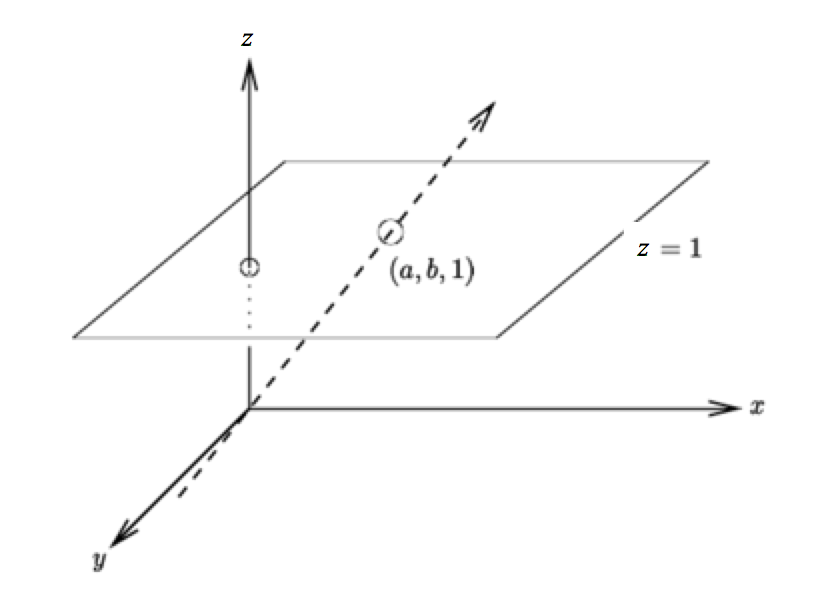
\includegraphics[width=0.6\textwidth]{images/ravnina.png}
% \caption[caption za v kazalo]{Dolg caption pod sliko}
  \caption[Primer točke v projektivni ravnini.]{Točka [a,b,1] v projektivni ravnini.}
  \label{fig:ravnina}
\end{figure}


\begin{definicija}~

Polinom $P$ je \emph{homogen} stopnje $d$, če velja $P(\lambda x,\lambda y, \lambda z) = \lambda ^d P(x,y,z)$ za vse $\lambda \in \F$.
\end{definicija}

\begin{definicija}~

\emph{Algebraična krivulja}, podana s homogenim polinomom $P$, je množica točk 
$$\mathcal{C}_P= \{ A \in \mathbb{P}^2, P(A) = 0 \}.$$
\end{definicija}

\emph{Kubična krivulja} je algebraična krivulja, podana s homogenim polinomom stopnje 3. V splošnem je torej oblike
\begin{align}
&{} a_{300}x^3+a_{210}x^2y+a_{201}x^2z+a_{120}xy^2+a_{102}xz^2+ \nonumber \\
&{}+a_{012}yz^2+a_{030}y^3+a_{003}z^3+a_{111}xyz+a_{021}y^2z = 0, \nonumber
\end{align}
kjer so $a_{ijk} \in \F$.
Ta zapis vsebuje $10$ koeficientov, vendar se v gladkih primerih lahko polinom poenostavi.
\begin{definicija}~\\
Algebraična krivulja je \emph{gladka}, če nima nobenih samopresečišč ali singularnosti.
\end{definicija}

\begin{izrek}[\protect{\cite{gibson}, Izrek 15.2}]~

Gladko kubično krivuljo nad algebraično zaprtim poljem lahko zapišemo v Weierstrassovi obliki
$$y^2z = x^3 + axz^2 + bz^3.$$
\end{izrek}

\begin{primer}~

Polinom $P(x,y,z) = z^2y-x^3$ je homogen polinom stopnje $3$. Rešitve enačbe $z^2y-x^3 = 0$ pa podajajo točke na kubični krivulji.
\\


\begin{figure}[ht]
  \centering
\begin{minipage}{.5\textwidth}
  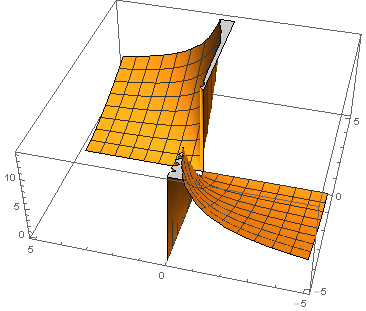
\includegraphics[width=0.8\textwidth]{images/krivulja.png}
  \caption[Primer algebraične krivulje.]{Algebraična krivulja, podana s polinomom $z^2y-x^3$.}
  \label{fig:krivulja}
\end{minipage}%
\begin{minipage}{.5\textwidth}
\centering
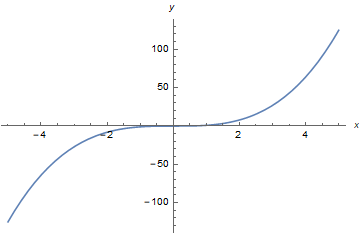
\includegraphics[scale=0.5]{images/projektivnaz.png}
\caption[Presek algebraične krivulje z ravnino $z=1$.]{Presek algebraične krivulje z ravnino $z=1$.}
\label{fig:projektivnaz}
\end{minipage}
\end{figure}


\begin{figure}[ht]
\centering
\begin{minipage}{.5\textwidth}
\centering
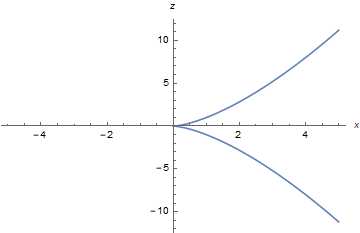
\includegraphics[scale=0.5]{images/projektivnay.png}
\caption[Presek algebraične krivulje z ravnino $y=1$.]{Presek algebraične krivulje z ravnino $y=1$.}
\label{fig:projektivnay}
\end{minipage}%
\begin{minipage}{.5\textwidth}
\centering
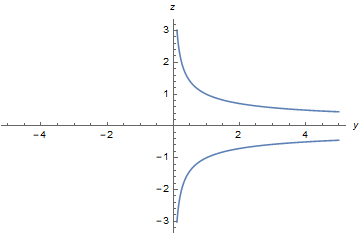
\includegraphics[scale=0.5]{images/projektivnax.png}
\caption[Presek algebraične krivulje z ravnino $x=1$.]{Presek algebraične krivulje z ravnino $x=1$.}
\label{fig:projektivnax}
\end{minipage}
\end{figure}


Na zgornjih slikah lahko vidimo, kako krivuljo predstavimo v projektivni ravnini, ter njene preseke z različnimi afinimi ravninami.

\end{primer}



V nadaljevanju nas bodo zanimale predvsem gladke kubične krivulje v polju $\mathbb{Z}/n\mathbb{Z}$.

\begin{definicija}~
Za dani števili $a$, $b \in \mathbb{Z}/n\mathbb{Z}$ je \emph{kubična krivulja} nad poljem $\mathbb{Z}/n\mathbb{Z}$ množica točk
$$E_{(a,b)}(\mathbb{Z}/n\mathbb{Z}) =\left\{ [x,y,z] \in \PP^2(\mathbb{Z}/n\mathbb{Z}): y^2z=x^3+axz^2+bz^3 \right\} .$$
Drugače povedano, afina kubična krivulja je množica rešitev enačbe
$$y^2=x^3+ax+b.$$
Pri čemer upoštevamo zvezo med afinimi in projektivnimi koordinatami točk:
$$(x,y)\in (\Z/n\Z)^2 \Leftrightarrow [x,y,1]\in \PP^2(\Z/n\Z).$$

\end{definicija}
\newpage
\subsection{Struktura grupe na kubičnih krivuljah}
Za definicijo grupe na kubičnih krivuljah uvedimo najprej pomožno operacijo

$$\ast : \mathcal{C}_P \times \mathcal{C}_P \rightarrow \mathcal{C}_P,$$
tako da za poljubni točki $A$, $B$ na krivulji velja:

\[ A \ast B =
\begin{cases}
A & \quad \text{če je } A=B \ \text{prevoj},\\
C & \quad \text{če je } \overline{AB} \cap \mathcal{C}_P = \left\{ A,B,C \right\},\\
A & \quad \text{če je } \overline{AB} \ \text{tangenta v } A,\ \text{ter} \ A \neq B,\\
B & \quad \text{če je } \overline{AB} \ \text{tangenta v } B,\ \text{ter} \ A \neq B,\\
C &\quad \text{če je } A=B \ \{\text{in tangenta v A}\} \cap \mathcal{C}_P = \left\{ A,C \right\}.\\
\end{cases}
\]
Intuitivno operacija $\ast$ vrne tretjo točko v preseku premice skozi $A$ in $B$ in $\mathcal{C}_P$. Poglejmo si še nekaj lastnosti operacije $\ast$. Dokaze sledečih trditev najdemo v \cite[Poglavje 17.3]{gibson}.

\begin{trditev}~

\label{last zvezda}
Operacija $\ast$ ima naslednje lastnosti:

\begin{itemize}
\item komutativnost: $ A \ast B = B \ast A$,
\item absorpcija: $(A \ast B ) \ast A = B$ ,
\item $((A \ast B) \ast C ) \ast D = A \ast ((B \ast D)\ast C)$.
\end{itemize}
\end{trditev}

\begin{izrek}~

Kubična krivulja ($\mathcal{C}_P$,$+$) je Abelova grupa za operacijo

\begin{table}[ht]
\centering
\begin{tabular}{llll}
$+:$ & $\mathcal{C}_P \times \mathcal{C}_P$ & $\rightarrow$ & $\mathcal{C}_P$ \\
& $(A,B)$ & $\rightarrow$ & $(A\ast B)\ast O$ ,
\end{tabular}
\end{table}
kjer je $O$ poljubna izbrana točka na krivulji $ \mathcal{C}_P$.
\end{izrek}

\begin{proof}~

S pomočjo trditve \ref{last zvezda} dokažimo, da je ($\mathcal{C}_P$,$+$) res Abelova grupa.

\begin{itemize}
\item Operacija $+$ je komutativna:
$$A+B = (A \ast B ) \ast O = (B \ast A) \ast O = B+A.$$
\item Točka O je nevtralni element:
$$A+O=(A \ast O) \ast O = A.$$
\item Nasprotni element A definiramo kot $-A = A \ast (O \ast O )$ in preverimo:
\begin{align}
A + (-A) &{} = (A \ast (A \ast (O \ast O))) \ast O \nonumber \\
&{} = (O \ast O) \ast O \nonumber \\
&{} = O, \nonumber
\end{align}
kjer smo uporabili absorbcijo.
\item Asociativnost $(A + B) + C = A + (B + C)$ dokažemo z računom:
\begin{align}
(A + B) + C &{} = ((A + B) \ast C) \ast O \nonumber \\
&{} = (((A \ast B) \ast O) \ast C) \ast O \nonumber \\
&{} = (A \ast ((B \ast C) \ast O)) \ast O \nonumber \\
&{} = (A \ast (B + C)) \ast O = A + (B + C). \nonumber \qedhere
\end{align}
\end{itemize}
\end{proof}

Ta definicija operacije nudi eleganten opis strukture grupe, za numerično računanje pa ni primerna. Možno pa je izpeljati formule, s katerimi lahko eksplicitno
izračunamo vsoto dveh točk, v kolikor imamo kubično krivuljo v Weierstrassvi obliki.

\begin{lema}[Seštevanje točk na Weierstrassovi kubični krivulji]~

\label{sestevanje}
Naj bo $\mathcal{C}_P$ afina krivulja v Weierstrassovi obliki $y^2 = x^3 + \alpha x^2 + \beta x + \gamma$, ter $O$ prevoj v neskončnosti. Če sta $A_1 = (a_1,b_1)$ in $A_2 = (a_2,b_2)$ točki na afinem delu $\mathcal{C}_P$, potem za $A_3 = A_1 + A_2 = (a_3,b_3)$ velja

\begin{align}
&{} a_3 = \lambda ^2 - \alpha - a_1 - a_2 \nonumber \\
&{} b_3 = -\lambda a_3 - \mu, \nonumber
\end{align}
kjer sta 

\[ \lambda =
\begin{cases}
\frac{b_1 - b_2}{a_1 - a_2} & \quad \text{če } a_1 \neq a_2 ,\\
\frac{3a_1^2+ 2 \alpha a_1 + \beta}{2b_1} & \quad \text{sicer} ,\\
\end{cases}
\]

ter $\mu = b_1 - \lambda a_1$.

\end{lema}


\begin{opomba}
Če krivuljo $\mathcal{C}_P$ predstavimo v projektivni ravnini, torej s homogenim polinomom $yz^2=x^3+\alpha x^2z+\beta xz^2+ \gamma yz^2$ je prevoj $O=[0,1,0].$
\end{opomba}

\begin{primer}~

Na spodnji sliki je v afini ravnini $y=1$ prikazano kako grafično seštevamo točke na Weierstrassovi kubiki $yz^2-x(x-y)(x+y)=0$. Sešteti želimo točki $A =(-1,0)$ in $B=(2,\sqrt{6}) $.
\\


\begin{figure}[h]
  \centering
  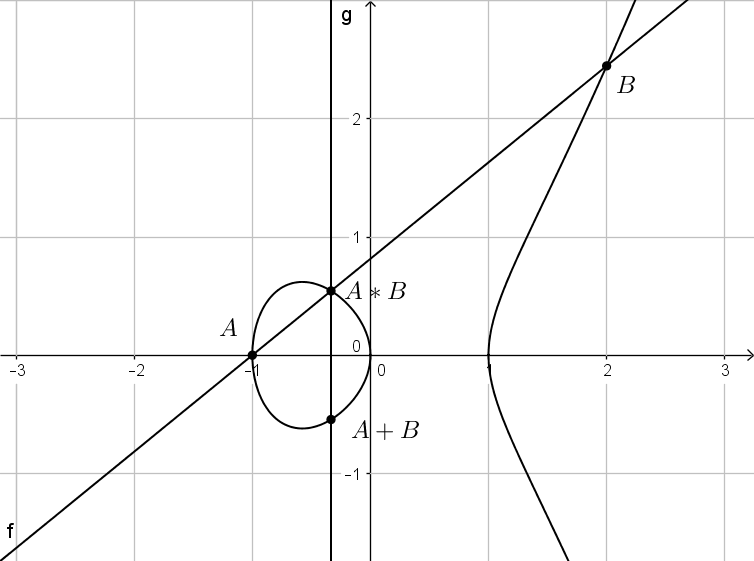
\includegraphics[width=0.8\textwidth]{images/adicija.png}
  \caption[Grafično seštevanje.]{Grafično seštevanje točk na kubični krivulji.}
  \label{fig:adicija}
\end{figure}

\end{primer}



\begin{primer}~

Seštejmo točki $A =(-1,0),B=(2,\sqrt{6}) $ na Weierstrassovi kubični krivulji $yz^2-x(x-y)(x+y)=0$ v preseku s projektivno ravnino $y=1$ še računsko z uporabo zgornje leme \ref{sestevanje}.
Prepišimo našo krivuljo najprej v afino obliko iz leme \ref{sestevanje}. Ker smo v ravnini $y=1$, najprej zamenjajmo vlogi $y$ in $z$.

$$z^2-x(x-1)(x+1) = 0 $$ 
Dobimo $z^2 = x^3-x,$
torej je $\alpha = 0$, $\beta = -1$ in $\gamma=0$. Izračunajmo sedaj $\lambda$ in $\mu$, pri čemer upoštevamo prvi predpis, saj sta x-koordinati točk različni:
$$\lambda = \frac{-\sqrt{6}}{-1-2} = \frac{\sqrt{6}}{3},$$

$$\mu = 0 - \frac{\sqrt{6}}{3} (-1) = \frac{\sqrt{6}}{3}.$$

Koordinati vsote $A+B=(x,y)$ sta torej enaki

$$x = \frac{6}{9} - 0+1-2=-\frac{1}{3}$$

in

$$z = -\frac{\sqrt{6}}{3}(-\frac{1}{3})-\frac{\sqrt{6}}{3}=-\frac{2\sqrt{6}}{9} \doteq -0.5443.$$

Iskana točka $A+B \in \PP^2$ je torej enaka $[-\frac{1}{3},1,-\frac{2\sqrt{6}}{9}]$. Dobljeni rezultat se ujema s točko, ki smo jo dobili z grafičnim seštevanjem.

\end{primer}

%%%%%%%%%%%%%%%%%%%%%%%%%%%%%%%%%%%%%%%%%%%%%%%%%%%%%%%%%%%%%%%%%%%%%%%%%%%%%%%%%%%%%%
%DIEFFIE-HELLMAN
%%%%%%%%%%%%%%%%%%%%%%%%%%%%%%%%%%%%%%%%%%%%%%%%%%%%%%%%%%%%%%%%%%%%%%%%%%%%%%%%%%%%%%

\section{Diffie-Hellmanova izmenjava ključev nad gladkimi kubičnimi krivuljami}

Diffe-Hellmanova izmenjava ključev je postopek, pri katerem se dve osebi npr.\  Alenka in Boris dogovorita za skrivni ključ na takšen način, da tudi v primeru ko njun pogovor posluša tretji nepovabljeni gost npr.\  Ciril le ta iz pogovora ne more rekonstruirati ključa za katerega sta se tekom pogovora dogovorila Alenka in Boris. 
\begin{algorithm}[H]
\caption[Diffe-Hellman]{Diffie-Hellmanova izmenjava ključev.}
\label{alg:diffie-hellman}

\begin{enumerate}

\item Alenka in Boris se dogovorita za elitpično krivuljo $E$ nad končnim obsegom $\F{q}$, ter za točko $P \in \E{\Fq{q}}$.
\item Alenka se odloči za skrivno število $a \in \N$, in izračuna $P_a = aP$, ter to pošlje Borisu.
\item Boris se odloči za skrivno število $b \in \N$, in izračuna $P_b = bP$, ter to pošlje Alenki.
\item Alenka izračuna $aP_b=abP$.
\item Boris izračuna $bP_a=baP$.

\end{enumerate}
\end{algorithm}

Kot sam ključ bi lahko na koncu Alenka in Boris uporabila npr.\  zadnjih $256$ bitov x-koordinate točke $abP$. Tu se zanašamo na to, da je iz $E, \F{q},P, P_a, P_b$ težko izračunati $baP$. Zelo veliko pa je tu odvisno od same izbire krivulje E.

To nas privede do t.\ i.\ problema diskretnega logaritma.


\begin{definicija}~
Naj bosta $a, b \in \N$, ter naj bo p praštevilo. Iščemo število k tako, da bo
$$a^k \equiv b\ (\text{mod} \ p).$$
\end{definicija}

\begin{trditev}~
Če lahko rešimo problem diskretnega logaritma, potem smo rešili tudi problem Diffie-Hellmanove izmenjave ključev. Povedano drugače velja
$$\text{DL} \Rightarrow DH.$$
\end{trditev}

\begin{proof}
Problem Diffie-Hellmanove izmenjave ključev lahko enostavno prevedemo na problem diskretnega logaritma na sledeč način:

\begin{itemize}
\item Vzemi $aP$ in izračunaj $a$ tako, da rešiš problem diskretnega logaritma.
\item Izračunaj $a(bP)$.
\end{itemize}

\end{proof}

\subsection{Index Calculus}
\label{IndexCalc}

Naj bo $p$ praštevilo in naj bo $g$ generator ciklične grupe $\F^{\times}_{p}$. Naj $L(h)$ označuje vrednost, za katero velja
$$g^{L(h)} \equiv h \ (\text{mod} \ p).$$
Iz definicije $L(h)$ sledi, da velja $$L(h_1h_2) = L(h_1)+L(h_2) \ (\text{mod} \ p).$$
Idejo napada na problem diskretnega logaritma v taki grupi najlažje vidimo na primeru.

\begin{primer}
Naj bo $p = 1217$ in $g= 3$. Rešiti hočemo $3^k \equiv 37 \mod 1217$. Izberimo si bazo praštevil $\{ 2,3,5,7,11,13 \}$. Pri tem upoštevamo, da bo večja baza pomenila več računanja a hkrati lažjo pot do odgovora. Išemo $x$-e  tako, da bo
$$3^x \equiv \pm \text{produktu praštevil iz baze} \mod 1217.$$

Ob iskanju takih $x$ najdemo naslednje enakosti:
\begin{align}
3^1 &\equiv 3 \MOD{1217} \nonumber \\ 
3^{24}  &\equiv -2^2\cdot 7\cdot 13 \MOD{1217} \nonumber \\
3^{25}  &\equiv 5^3 \MOD{1217} \nonumber \\
3^{30}  &\equiv -2 \cdot 5^2 \MOD{1217} \nonumber \\
3^{54}  &\equiv -5\cdot 11 \MOD{1217} \nonumber \\
3^{87}  &\equiv 13 \MOD{1217} \nonumber
\end{align}
Z večjo bazo bi v tem primeru lažje našli take enačbe, a bi jih hkrati potrebovali več.
Z uporabo malega Fermatovega izreka, velja
$$3^{1216} \equiv 1 \equiv (-1)^2 \mod 1217, $$
od koder sledi $L(-1) \equiv 608 \mod 1216$.
Če enačbe sedaj zapišemo z uporabo $L(h)$, dobimo
\begin{align}
1 &\equiv L(3) \MOD{1216} \nonumber \\ 
24&\equiv 608 + 2L(2) + L(7) +L(13) \MOD{1216} \nonumber \\
25 &\equiv 3L(5) \MOD{1216} \nonumber \\
30 &\equiv 608+L(2)+2L(5) \MOD{1216} \nonumber \\
54 &\equiv 608+L(5)+L(11) \MOD{1216} \nonumber \\
87  &\equiv L(13) \MOD{1216}  \nonumber
\end{align}

Od tod bobimo $L(2) = 216, L(11)=1059,L(7) = 113,L(5) = 819,L(13) = 87,L(3)=1$.
Sedaj poračunamo za različne $j$ vrednost $3^j*37$, dokler ne dobimo $3^j*37 \equiv \text{produktu elementov iz baze}$.
Pri vrednosti $j=16$ dobimo
$$3^{16}\cdot 37 \equiv 2^3\cdot 7 \cdot 11 \MOD{1217}.$$
Iščemo $L(37)$, iz definicije $L$ pa velja
$$3^{L(37)} \equiv 37 \MOD{1217} \equiv 2^3\cdot 7 \cdot 11 \cdot 3^{-16}\MOD{1217}.$$
Če sedaj namesto baze vstavimo primerne $L$ dobimo
$$3^{L(37)} \equiv 3^{3L(2)}\cdot 3^{L(7)} \cdot 3^{L(11)} \cdot 3^{-16L(3)}\MOD{1217}.$$
$L(37)$ lahko sedaj zapišemo kot
$$L(37) \equiv 3L(2) +L(7)+L(11) - 16L(3) \MOD{1216} \equiv 588 \MOD{1216}.$$

Torej je naš iskani $k=588$.

\end{primer}

%%%%%%%%%%%%%%%%%%%%%%%%%%%%%%%%%%%%%%%%%%%%%%%%%%%%%%%%%%%%%%%%%%%%%%%%%%%%%%%%%%%%%%
%PARJENJA
%%%%%%%%%%%%%%%%%%%%%%%%%%%%%%%%%%%%%%%%%%%%%%%%%%%%%%%%%%%%%%%%%%%%%%%%%%%%%%%%%%%%%%
\section{Parjenja}

Parjenja imajo pomembno vlogo pri napadih na problem diskretnega logaritma nad gladkimi kubičnimi krivuljami.

\begin{definicija}~
\emph{Eliptična} krivulja je gladka kubična krivulja.
\end{definicija}

\begin{definicija}~
Naj bo $E$ eliptična krivulja nad poljem $K$, ter naj bo $n\in \N$. \emph{Torizjske točke} so množica
$$E[n] = \{ P \in \E{\overline{K}} | nP = \infty \}.$$
\end{definicija}

\begin{izrek}
\label{IzrekTor}
Naj bo $E$ eliptična krivulja nad poljem $K$ in naj bo $n \in \N$. Če karakteristika polja $K$ ne deli $n$, ali je enaka $0$ potem
$$E[n] \cong \mathbb{Z}_n \oplus \mathbb{Z}_n$$

\end{izrek}

\begin{proof}
Se ne vem kako bo napisan
\end{proof}

\begin{definicija}~
Definirajmo \emph{deliteljski polinom} $\gamma_m \in \Z[x,y,A,B]$ kot,


\begin{align}
\gamma_0 &{}= 0  \nonumber \\
\gamma_1 &{}= 1  \nonumber \\
\gamma_2 &{}= 2y  \nonumber \\
\gamma_3 &{}= 3x^4 + 6Ax^2 + 12Bx-A^2 \nonumber \\
\gamma_4 &{}= 4y(x^6+5Ax^4+20Bx^3-5A^2x^2-4ABx-8B^2-A^3) \nonumber \\
\gamma_{2m+1} &{}= \gamma_{m+2}\gamma_{m}^3-\gamma_{m-1}\gamma_{m+1}^3 \text{za } m \geq 2 \nonumber \\
\gamma_{2m} &{}= (2y)^{-1}\gamma_{m}(\gamma_{m+2}\gamma_{m-1}^2-\gamma_{m-2}\gamma_{m+1}^2)\text{za } m \geq 3 \nonumber
\end{align}

\end{definicija}

\begin{lema}

$\gamma_{n}$ je element $\Z[x,y^2,A,B]$, za vse lihe $n$.  Za sode $n$ pa je $\gamma_{n}$ element $2y\Z[x,y^2,A,B]$.

\end{lema}

\begin{proof}
Dokažimo to s pomočjo indukcije. Za $n \leq 4$ lema očitno velja. Obravnavajmo primera, ko je $n=2m$ in  $n=2m+1$ za nek $m\in\N$.
\begin{itemize}
\item{n=2m}
Indukcijska predpostavka je v tem primeru, da lema velja za vse $n<2m$.
Predpostavimo lahko, da je $2m>4$, saj vemo da lema velja za $n\leq 4$, torej velja $m>2$. Potem velja $2m>m+2$, kar pomeni, da vsi polinomi v definiciji $\gamma_{2m}$ zadoščajo indukcijski predpostavki. Če je $m$ sodo število ,potem se $\gamma{m},\gamma{m+2},\gamma{m-2}$ nahajajo v $2y\Z[x,y^2,A,B]$. Od tod pa sledi, da je tudi $\gamma_{2m} \in 2y\Z[x,y^2,A,B]$.
Če je $m$ lih, potem sta $\gamma{m-1},\gamma{m+1} \in 2y\Z[x,y^2,A,B]$. To pa pomeni, da je tudi  $\gamma_{2m} \in 2y\Z[x,y^2,A,B]$.
\item{n=2m+1}
Primer obravnavamo podobno kot $n=2m$.


\end{itemize}


\end{proof}

\begin{definicija}~
Naj bo $K$ polje in naj bo $n \in \N$ tak, da karakteristika $K$ ne deli $n$.
$$\mu_n = \{ x \in \overline{K} | x^n = 1 \}$$
je \emph{grupa n-tih korenov enote} grupe $\overline{K}$.
\end{definicija}

\begin{trditev}
\label{trd-WeilPar}
Naj bo E eliptična krivulja definirana nad poljem $K$, in naj bo $n \in \N$. Predpostavimo, da karakteristika polja $K$ ne deli $n$. Potem obstaja Weilovo parjenje
$$e_n:E[n] \times E[n] \rightarrow \mu_n,$$
za katerega velja:
\begin{itemize}
\item $e_n$ je bilinearna v obeh spremenljivkah
$$e_n(S_1+S_2,T) = e_n(S_1,T)e_n(S_2,T)$$
in
$$e_n(S,T_1+T_2) = e_n(S,T_1)e_n(S,T_2)$$
za vse $S,S_1,S_2,T,T_1,T_2 \in E[n]$.
\item $e_n$ je nedegenerirana v obeh spremenljivkah. To pomeni če je $e_n(S,T) = 1$ za vse $T \in E[n]$ potem $S = \infty$, ter obratno.

\item $e_n(T,T) = 1$ za vse $T \in E[n]$

\item $e_n(T,S) = e_n(S,T)^{-1}$ za vse $S,T \in E[n]$

\item $e_n(\rho S,\rho T) = \rho(e_n(S,T))$ za vse avtomorfizme $\rho$ iz $\bar{K}$, za katere je $\rho$ identiteta na koeficientih $E$.

\item $e_n(\alpha(S),\alpha(T)) = e_n(S,T)^{\text{deg}(\alpha)}$ za vse separabilne endomorfizme $\alpha$ polja $E$.
\end{itemize}

\end{trditev}


\begin{posledica}
\label{PosledicaTrdParj}
Naj bosta $T_1,T_2$ baza $E[n]$. Potem je $e_n(T_1,T_2)$ generator grupe $\mu_N$.
\end{posledica}

\begin{proof}
Vemo, da za poljubni točki $T_1,T_2$ velja $e_n(T_1,T_2)^n = 1$, ker se slika parjenja nahaja v grupi $n$-tih korenov enote. Pokazati moramo torej, da če za neko število $d$ velja  $e_n(T_1,T_2)^d = 1$ potem od tod sledi, da je $d \geq n$.
Recimo torej, da je $e_n(T_1,T_2) = \zeta$, kjer velja $\zeta^d = 1$.
Po točki ena trditve \ref{trd-WeilPar} velja $$e_n(T_1,dT_2) = e_n(T_1,T_2)^d=1.$$ Prav tako velja $e_n(T_2,dT_2) = e_n(T_2,T_2)^d = 1 $. Naj bo $S \in E[n]$, potem se $S$ izraža kot $S = aT_1+bT_2$ za neka $a,b \in \N$.
S ponovno uporabo trditve \ref{trd-WeilPar} vidimo, da velja
$$e_n(S,dT_2)= e_n(T_1,dT_2)^ae_n(T_2,dT_2)^b = 1. $$
Ker to valja za vsak $S$ po točki dva trditve \ref{trd-WeilPar} sledi, da je $dT_2 = \infty$. To pa je mogoče le če $n|d$, kar pomeni da je $n \leq d$.
\end{proof}

%%%%%%%%%%%%%%%%%%%%%%%%%%%%%%%%%%%%%%%%%%%%%%%%%%%%%%%%%%%%%%%%%%%%%%%%%%%%%%%%%%%%%%
%MOV
%%%%%%%%%%%%%%%%%%%%%%%%%%%%%%%%%%%%%%%%%%%%%%%%%%%%%%%%%%%%%%%%%%%%%%%%%%%%%%%%%%%%%%

\section{MOV}
MOV napad s pomočjo Weilovega parjenja pretvori problem diskretnega logaritma iz $E(\F{q})$ v problem diskretnega logaritma nad $\F^{\times}_{q^m}$. Na ta način se izognemo težji strukturi grupe. Nov problem diskretnega logaritma pa lahko sedaj rešimo z različnimi napadi, med drugim tudi z napadom Index-Calculus \ref{IndexCalc}. MOV napad deluje če velikost polja $\F{q^m}$ ni dosti večja od velikosti polja $\F{q}$. Postopek napada sledi poteku dokaza naslednje trditve.

\begin{trditev}
Naj bo $E$ eliptična krivulja nad $\F{q}$. Naj bosta $P,Q \in E(\F{q})$, ter naj bo $N$ red točke $P$. Predpostavimo, da velja $\text{gcd}(N,q)=1$. Potem obstaja tako število $k$, da velja $Q = kP$ natanko tedaj ko $NQ = \infty$ in $e_N(P,Q)=1$.
\end{trditev}

\begin{proof}
$(\Rightarrow)$ Če je $Q = kP$, potem je $NQ = kNP$, ampak ker je red $P$ enak $N$ od tod sledi $kNP = \infty$. Prav tako
$$e_n(P,Q) = e_n(P,P)^k = 1^k = 1.$$

$(\Leftarrow)$ Naj bo $NQ = \infty$, torej je po definiciji $Q \in E[N]$. Ker je $\text{gcd}(N,q) = 1$ lahko uporabimo izrek \ref{IzrekTor} in zapišemo 
$E[N] \cong \Z_N \oplus \Z_n$. Sedaj izberemo točko $R$ tako, da je $\{P,R \}$ baza $E[N]$. Ker sta $P,R$ baza  lahko $Q$ zapišemo kot
$$Q = aP+bR,$$
za neki števili $a,b \in \N$. Po posledici definicije Weilovega parjenja \ref{PosledicaTrdParj} velja 

\noindent $e_N(P,R)=\zeta$ je generator $\mu_N$.
Po predpostavki velja $e_N(P,Q) = 1$ dobimo torej
$$1 = e_N(P,Q) = e_N(P,P)^ae_N(P,R)^b = \zeta^b.$$
Od tod sledi, da je $b$ večkratnik števila $N$, od tod pa po definiciji sledi $bR = \infty$, ter $Q = aP$.
\end{proof}

Ideja dokaza nam sedaj, da korake MOV napada.

\begin{algorithm}[H]
\caption[MOV]{MOV napad}
\label{alg:MOV}
Izberi $m$ tako, da $$E[N] \subset \E{\F{q^n}}.$$
Ker imajo vse točke $E[N]$ koordiante v $\bar{\F{q}} = \cup_{j\geq 1}\F_{q^j}$ tak $m$ obstaja. Prav tako je $\mu_N$ v $\F{q^m}$.
Nato postopaj po naslednjih korakih.
\begin{enumerate}
\item Izberi točko $T \in \E{\F{q^m}}$.
\item Izračunaj red $M$ točke $T$.
\item Naj bo $d = \text{gcd}(M,N)$ in naj bo $T_1 = (M/d)T$. Potem ima $T_1$ red, ki deli $N$, torej je $T_1 \in E[N]$.
\item Izračunaj $\zeta_1 = e_N(P,T_1)$ in $\zeta_2 = e_N(Q,T_1)$. Tu sta $\zeta_1$ in $\zeta_2$ v $\mu_d \subset \F_{q^m}^\times$.
\item Reši problem diskretnega logaritma $\zeta_2 = \zeta_1^k$ v $\F_{q^m}^\times$. To nam da $k \mod d$.
\item Ponovi korake $1$-$5$ za različnke točke $T$ dokler ni $k$ določen.
\end{enumerate}

\end{algorithm}
MOV napad deluje hitreje, kot če hočemo rešiti porblem diskretnega algoritma direktno nad krivuljo, če velja 
$$k > log^2(p),$$
kjer je krivulja $E(\F_p)$ in MOV pretvori to grupo v $\F^{\times}_{p^k}$.


\cite{Washington2008}
\cite{Silverman2009}

% Literatura:
% Primer navajanja na http://www.fmf.uni-lj.si/storage/24240/LiteraturaM.pdf,
% ampak bi moral stil poskrbeti za vse. Reference se uredijo po abecedi.
% Če nobena izbira izmed @book, @atricle,... ni ok, potem se lahko vse napiše v
% @misc pod note={} in deluje tako kot normalen LaTeX.
% Komentar v bib datoteki se naredi samo s parom { }
% Za urejanje literature avtor priporoča program Jabref, ki zna tudi avtomatsko
% okrajšati imena revij. Za pravilno sortiranje vnosov brez avtorja, uporabite
% polje key={ }, kot v primeru.
% V primeru napak ustvarite issue na GitHubu ali pišite na jure.slak@fmf.uni-lj.si.
\cleardoublepage                           % na desni strani
\phantomsection                            % da prav delujejo hiperlinki
\addcontentsline{toc}{section}{\bibname}   % dodajmo v kazalo
\bibliographystyle{fmf-sl}                 % uporabljen stil je v datoteki fmf-sl.bst, na voljo tudi angleška verzija
\bibliography{\literatura}                 % literatura je v datoteki, definirani na začetku

% Za stvarno kazalo
\cleardoublepage                           % na desni strani
\phantomsection                            % da prav delujejo hiperlinki
\addcontentsline{toc}{section}{\indexname} % dodajmo v kazalo
\printindex

\end{document}
